% Este archivo es parte de la memoria del proyecto fin de carrera
% de Manuel López Urbina. Protegida bajo la licencia GFDL.
% Para más información, la licencia completa viene incluida en el
% fichero fdl-1.3.tex

% Copyright (C) 2012 Manuel López Urbina

\chapter{Conceptos básicos}
\label{chap:conceptos-básicos}

\section{Vehículo Autónomo}
\label{sec:def-vehículo-autónomo}

Un vehículo autónomo, es un vehículo capaz de cumplir con las capacidades de transporte llevadas a cabo por los humanos en un vehículo tradicional por sí mismo. Dicho vehículo es capaz de detectar los diferentes elementos de su entorno permitiendo un desplazamiento por sí mismo. Un ser humano puede elegir un destino, siendo innecesario realizar ninguna otra operación mecánica en el vehículo.\\

Los Vehículos autónomos perciben el mundo que le rodea gracias a la utilización de multitud de sensores tales como radares, GPS y visión por computador, siendo esta última la principal temática de este proyecto. Posteriormente un sistema avanzados de control interpretará la información para identificar las rutas adecuadas de navegación, así como los obstáculos y la señalización correspondiente. Dichos vehículos suelen actualizar sus mapas basados en la información sensorial, de forma que permiten la navegación a través de entornos desconocidos.

\section{Inteligencia artificial}   
\label{sec:def-inteligencia-artificial}

La inteligencia artificial (IA) se define como la capacidad de un dispositivo para llevar a cabo funciones que normalmente se asocian con la inteligencia humana, tales como el razonamiento y la optimización de la experiencia. La IA es la rama de la informática que trata de aproximar los resultados del razonamiento humano mediante la organización y manipulando conocimiento de los hechos y heurísticos. Las áreas de actividad de AI incluyen los sistemas expertos, la comprensión del lenguaje natural, reconocimiento de voz, la visión artificial y la robótica.

\section{Visión artificial}
\label{def:visión-artificial}

La visión artificial, también conocida como visión por computador, es un subcampo perteneciente a la inteligencia artificial\footnote{Definición de \emph{inteligencia artificial} incluida en la sección \ref{sec:def-inteligencia-artificial}.}. El propósito de la visión artificial es programar un computador para que \emph{entienda} una escena o las características de una imagen.\\

Los objetivos típicos de la visión artificial incluyen:

\begin{itemize}
\item La detección, segmentación, localización y reconocimiento de objetos en imágenes (por ejemplo, caras humanas).
\item La evaluación de resultados (por ejemplo, segmentación, registro).
\item Registro de diferentes imágenes de una misma escena u objeto, es decir, hacer concordar un mismo objeto en diversas imágenes.
\item Seguimiento de un objeto en una secuencia de imágenes.
\item Mapeo de una escena para generar un modelo tridimensional de la escena; este modelo podría ser usado por un robot para navegar por la escena.
\item Búsqueda de imágenes digitales por su contenido.
\end{itemize}

Estos objetivos se consiguen por medio de reconocimiento de patrones\footnote{Definición de \emph{reconocimiento de patrones} disponible en la sección \ref{def:reconocimiento-de-patrones}.}, aprendizaje estadístico, geometría de proyección, procesamiento de imágenes, teoría de grafos y otros campos. En este proyecto nos centraremos en técnicas propias del reconocimiento de patrones.

\section{Reconocimiento de patrones}
\label{def:reconocimiento-de-patrones}

El reconocimiento de patrones, también llamado lectura de patrones, identificación de figuras y reconocimiento de formas, consiste en el reconocimiento de patrones de señales. Los patrones son obtenidos a partir de procesos de segmentación, extracción de características y descripción para que cada objeto quede representado de manera lo más representativa posible por una colección de descriptores. El sistema de reconocimiento debe asignar a cada objeto su categoría o clase (conjunto de entidades que comparten alguna característica que las hacen diferentes al resto). Para poder reconocer los patrones se siguen tres procesos principales:\\

\begin{itemize}
 \item Adquisición de datos.
 \item Extracción de características.
 \item Toma de decisiones.
\end{itemize}

La esencia del reconocimiento de patrones es la clasificación, un ejemplo práctico de clasificación puede ser la clasificación de imágenes digitales de letras en las clases de la \emph{A} a la \emph{Z} dependiendo de sus píxeles u otras situaciones que podamos extraer.\\

\begin{figure}[H]
  \begin{center}
    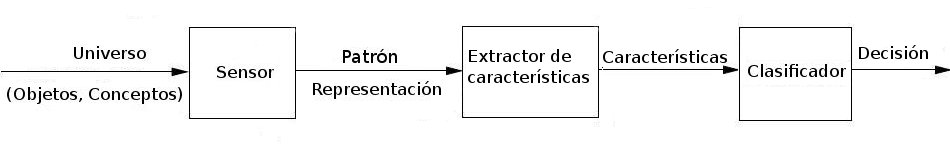
\includegraphics[scale=0.6]{Pattern.jpg}
  \end{center}
  \caption{Componentes básicos de un sistema de reconocimiento de patrones.}
  \label{Componentes-basicos-rp}
\end{figure}


\subsection {Aplicaciones}

Los sistemas de reconocimiento de patrones tienen multitud de aplicaciones. Algunas de las más relevantes y utilizadas actualmente son:\\

\begin{itemize}
\item Previsión meteorológica: poder clasificar datos meteorológicos según diversos patrones, y con el conocimiento a priori que tenemos de las diferentes situaciones que pueden aperecer nos permite crear mapas de predicción automática.
\item Reconocimiento de caracteres escritos a mano o a máquina: es una de las utilidades más populares de los sistemas de reconocimiento de patrones ya que los símbolos de escritura son fácilmente identificables.
\item Reconocimiento de voz: el análisis de la señal de voz se utiliza actualmente en muchas aplicaciones, un ejemplo claro son los teleoperadores informáticos.
\item Aplicaciones en medicina: análisis de biorritmos, detección de irregularidades en imágenes de rayos-x, detección de células infectadas, marcas en la piel...
\item Reconocimiento de huellas dactilares: utilizado y conocido por la gran mayoría, mediante las huellas dactilares todos somos identificables y con programas que detectan y clasifican las coincidencias, resulta sencillo encontrar correspondencias.
\item Reconocimiento de caras: utilizado para contar asistentes en una manifestación o simplemente para detectar una sonrisa, ya hay diferentes cámaras en el mercado con esta opción disponible.
Interpretación de fotografías aéreas y de satélite: gran utilidad para propuestas militares o civiles, como la agricultura, geología, geografía, planificación urbana...
\item Predicción de magnitudes máximas de terremotos.
\item Reconocimiento de objetos: con importantes aplicaciones para personas con discapacidad visual.
\item Reconocimiento de música: identificar el tipo de música o la canción concreta que suena.
\end{itemize}


\section {Modelos de color}
\label{def:modelos-color}

El color, como cualquier otro recurso, también tiene su técnica y se enecuntra sometido a ciertas leyes, y según la aplicación que se desea, se trabaja con distintos modelos de color. Los modelos de color describen los colores que se ven en las imágenes digitales e impresas y el trabajo con ellos.\\

Los modelos de color permiten, además de establecer un espacio único común a todos los equipos que realizan operaciones de adquisición y reproducción de color, permiten simular cómo lucirá la imagen y su color en otro dispositivo; así por ejemplo, podemos ver en la pantalla del computador cómo saldrá la imagen impresa en el papel, después de que haya pasado por las tintas que se usan normalmente en prensa y con diferentes papeles, permitiendo un trabajo de edición de imagen y color mucho más sencilla y fiel a los resultados finales.\\

Cada modelo de color como, por ejemplo, RGB, CMYK o HSV representa un método diferente (y por lo general, numérico) de descripción de los colores.\\

A continuación se describen los aquellos modelos de mayor importancia:

\subsection{Modelo RGB}

La descripción RGB, del inglés Red, Green, Blue, de un color hace referencia a la composición del color en términos de la intensidad de los colores primarios con que se forma: el rojo, el verde y el azul. Este modelo de color está basado en la síntesis aditiva, permitiendo representar un color mediante la mezcla por adición de los tres colores de luz primarios de los que se compone. El modelo de color RGB no define por sí mismo lo que significa exactamente rojo, verde o azul, por lo que los mismos valores RGB pueden mostrar colores notablemente diferentes en diferentes dispositivos que usen este modelo de color. Aunque utilicen un mismo modelo de color, sus espacios de color pueden variar considerablemente.
Con el fin de indicar con qué proporción se mezcla cada color, se asigna un valor numérico a cada uno de los colores primarios, de manera que, por ejemplo, el valor 0 significa que ese color no interviene en la mezcla y, a medida que ese valor aumenta, se entiende que aporta más intensidad al conjunto. Aunque el intervalo de valores podría ser cualquiera (valores reales entre 0 y 1, valores enteros entre 0 y 37, etc.), aunque en la mayoría de ocasiones cada color primario es codificado con un byte (8 bits). Así, de manera usual, la intensidad de cada una de las componentes se mide con una escala del 0 al 255.\\

Por lo tanto, el rojo es obtenido con (255,0,0), el verde con (0,255,0) y el azul con (0,0,255), siendo para los tres casos un color monocromático. La ausencia de color, lo que identificamos como el color negro, se obtiene cuando las tres componentes son 0, (0,0,0).\\

La combinación de dos colores a nivel 255 con un tercero en nivel 0 da lugar a la obtención de los tres colores intermedios. De esta forma el amarillo es (255,255,0), el cian (0,255,255) y el magenta (255,0,255).\\

Finalmente, el color blanco se forma con los tres colores primarios a su máximo nivel (255,255,255).\\

\begin{figure}[H]
  \begin{center}
    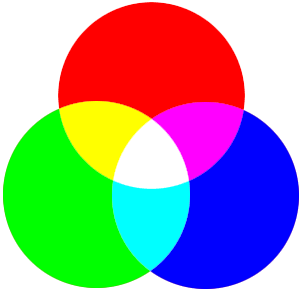
\includegraphics[scale=0.3]{modelo-RGB.png}
  \end{center}
  \caption{Modelo de color RGB.}
  \label{modelo-RGB}
\end{figure}

\subsection{Modelo HSV}

El modelo HSV, del inglés Hue, Saturation, Value que traducidos son,  Matiz, Saturación, Valor, se define como un modelo de color según sus componentes. Dicho modelo aplica una transformación no lineal sobre el espacio de color RGB, y se puede usar en progresiones de color.\\

\begin{figure}[H]
  \begin{center}
    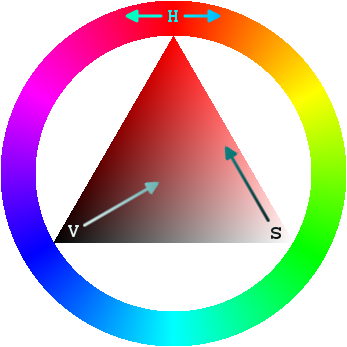
\includegraphics[scale=0.3]{triangulo-HSV.png}
  \end{center}
  \caption{Espacio de color HSV.}
  \label{modelo-RGB}
\end{figure}

\subsection{Uso}

Es común que deseemos elegir un color adecuado para alguna de nuestras aplicaciones, cuando es así resulta muy útil usar la ruleta de color HSV. En ella el matiz se representa por una región circular; una región triangular separada, puede ser usada para representar la saturación y el valor del color. Normalmente, el eje horizontal del triángulo denota la saturación, mientras que el eje vertical corresponde al valor del color. De este modo, un color puede ser elegido al tomar primero el matiz de una región circular, y después seleccionar la saturación y el valor del color deseados de la región triangular.\\

\subsection{Características}

Constituyentes en coordenadas cilíndricas:\\

\subsubsection{Matiz}

Se representa como un grado de ángulo cuyos valores posibles van de 0 a 360$^\circ$ (aunque para algunas aplicaciones se normalizan del 0 al 100 \%). Cada valor corresponde a un color. Ejemplos: 0 es rojo, 60 es amarillo y 120 es verde.
De forma intuitiva se puede realizar la siguiente transformación para conocer los valores básicos RGB:
Disponemos de 360 grados dónde se dividen los 3 colores RGB, eso da un total de 120$^\circ$ por color, sabiendo esto podemos recordar que el 0 es rojo RGB(1, 0, 0), 120 es verde RGB(0, 1, 0) y 240 es azul RGB(0, 0, 1). Para colores mixtos se utilizan los grados intermedios, el amarillo, RGB(1, 1, 0) está entre rojo y verde, por lo tanto 60$^\circ$. Se puede observar como se sigue la secuencia de sumar 60 grados y añadir un 1 o quitar el anterior:\\

\begin{itemize}
\item 0$^\circ$ = RGB(1, 0, 0)
\item 60$^{\circ}$ = RGB(1, 1, 0)
\item 120$^{\circ}$ = RGB(0, 1, 0)
\item 180$^{\circ}$ = RGB(0, 1, 1)
\item 240$^{\circ}$ = RGB(0, 0, 1)
\item 300$^{\circ}$ = RGB(1, 0, 1)
\item 360$^{\circ}$ = 0$^{\circ}$
\end{itemize}

Esta transformación permite saber los tonos de matices que contienen colores puros que contienen toda la cantidad (o ninguna) de los colores R, G y B. Para el color blanco puede poner cualquier matiz y establecer una saturación de 0. Por contra, para el color negro se puede poner cualquier color y saturación, siempre que se ponga un valor de 0.

\subsubsection{Saturación}

Se representa como la distancia al eje de brillo negro-blanco. Los valores posibles van del 0 al 100\%. Dicho parámetro también es conocido como ``pureza''. Cuanto menor sea la saturación de un color, mayor tonalidad grisácea tendrá y más decolorado estará.

\subsubsection{Valor}

El Valor es representativo de la altura en el eje blanco-negro. Los valores posibles varian del 0 al 100\%. 0 se corresponde con el negro. Dependiendo de la saturación, 100 podría ser blanco o un color más o menos saturado.

\subsection{Modelo CYMK}

El modelo CMYK, siendo acrónimo de Cyan, Magenta, Yellow y Key, es un modelo de color ampliamente utilizado en la impresión  de colores. Este modelo permite la representación de una amplia gama de colores y tiene una mejor adaptación a los medios industriales.\\

Este modelo se basa en la mezcla de pigmentos de los siguientes colores para crear otros más:\\

\begin{itemize}
\item C = Cyan (Cian).
\item M = Magenta (Magenta).
\item Y = Yellow (Amarillo).
\item K = Black o Key (Negro).
\end{itemize}

La mezcla de colores CMY ideales en un fondo blanco da como resultado el color negro aunque por diversar razones, el negro generado no es ideal. Por esta razón los dispositivos de impresión a cuatro tintas incorpora la de color negro.\\

\begin{figure}[H]
  \begin{center}
    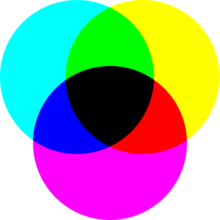
\includegraphics[scale=0.5]{CYMK.png}
  \end{center}
  \caption{Modelo de color CMYK.}
  \label{modelo-RGB}
\end{figure}
